\section{RESULTATS ET DISCUSSIONS}
\subsection{l'évaluation de l'impact de la NAO sur l'Upwelling}
\subsubsection{Analyse Générale}
une analyse de façon générale sur l’ensemble du pays montre que généralement le Maroc connaît l'upwelling dans la zone sud. Toutefois il est pertinent d'analyser le pays en entier pour détecter un éventuel impact des changement climatiques sur la situation dans le pays.
  
\begin{figure}[H]
\centering
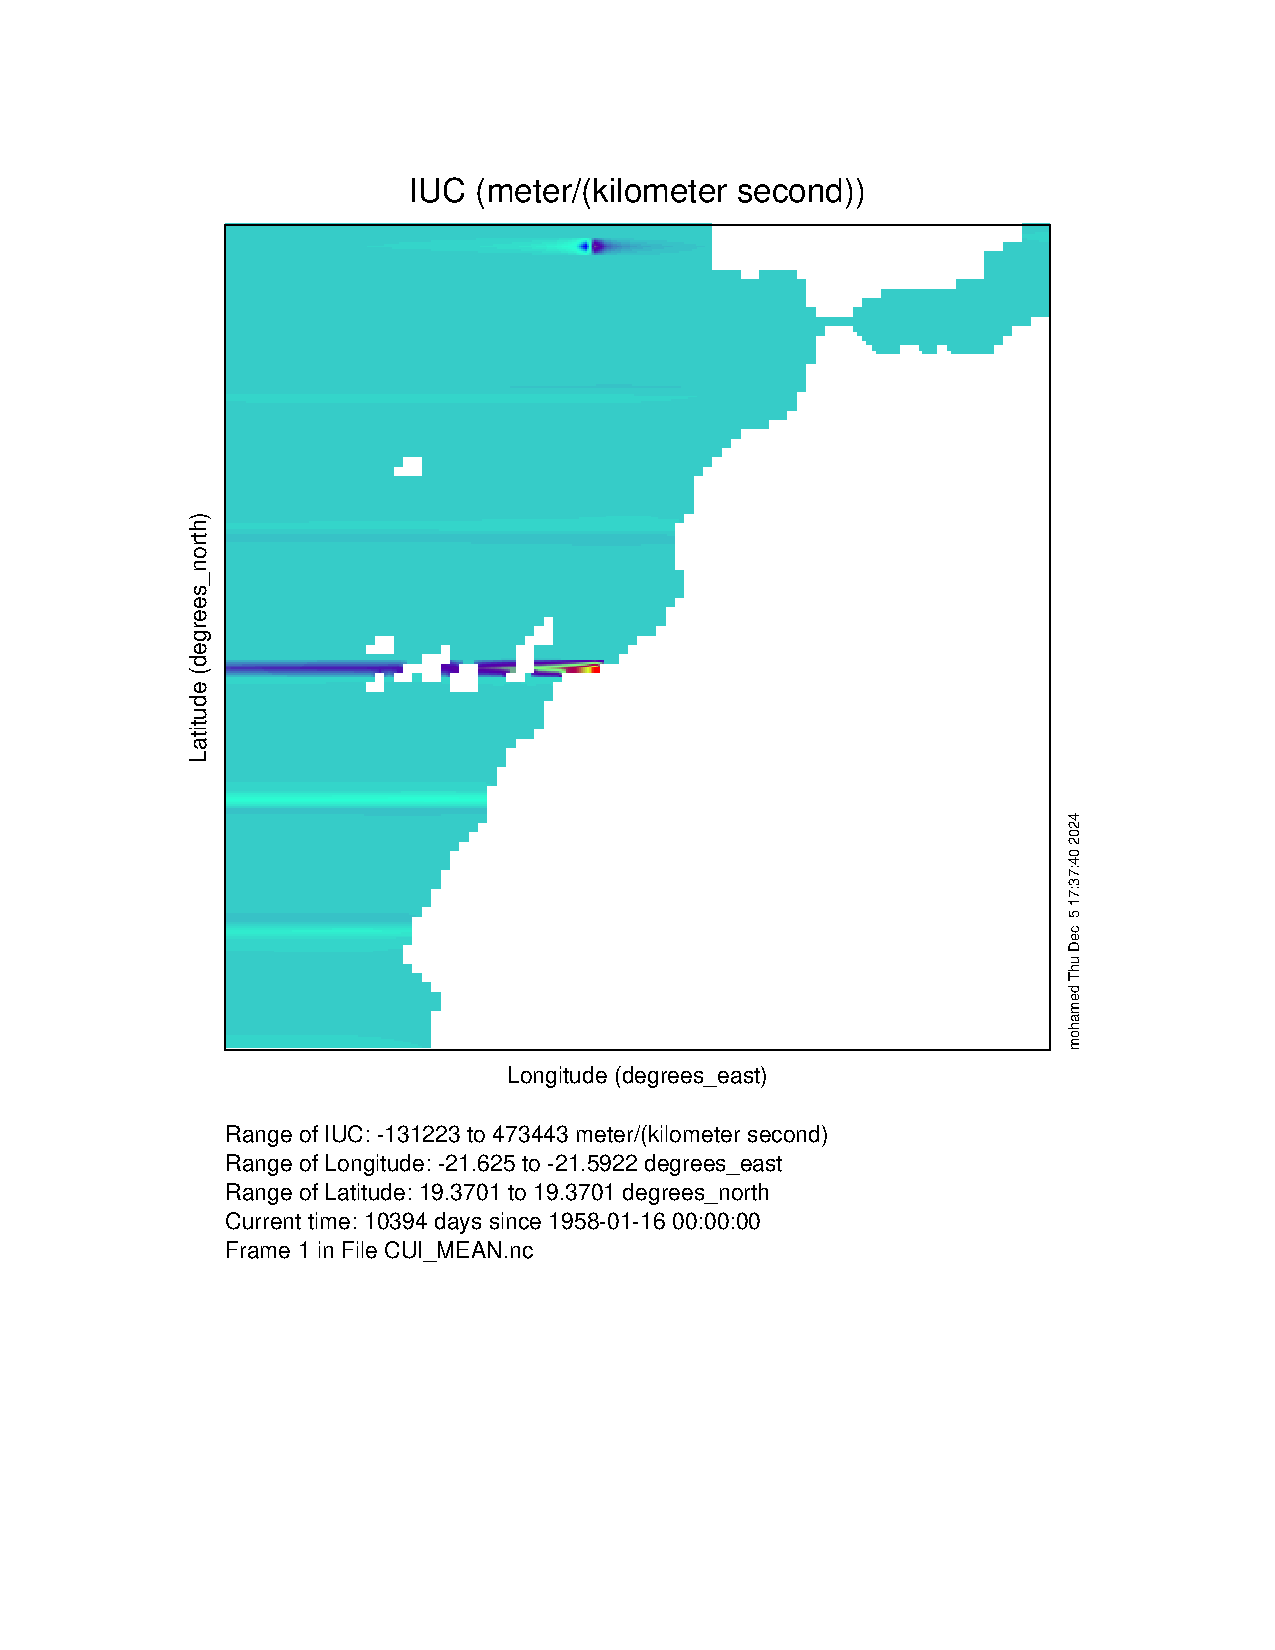
\includegraphics[scale=0.5]{ncview_output.pdf}
\caption{Climatologie de l'Upwelling au Maroc  1958-2014}
\end{figure}


\subsubsection{Analyse des distributions}

\begin{figure}[H]
\centering
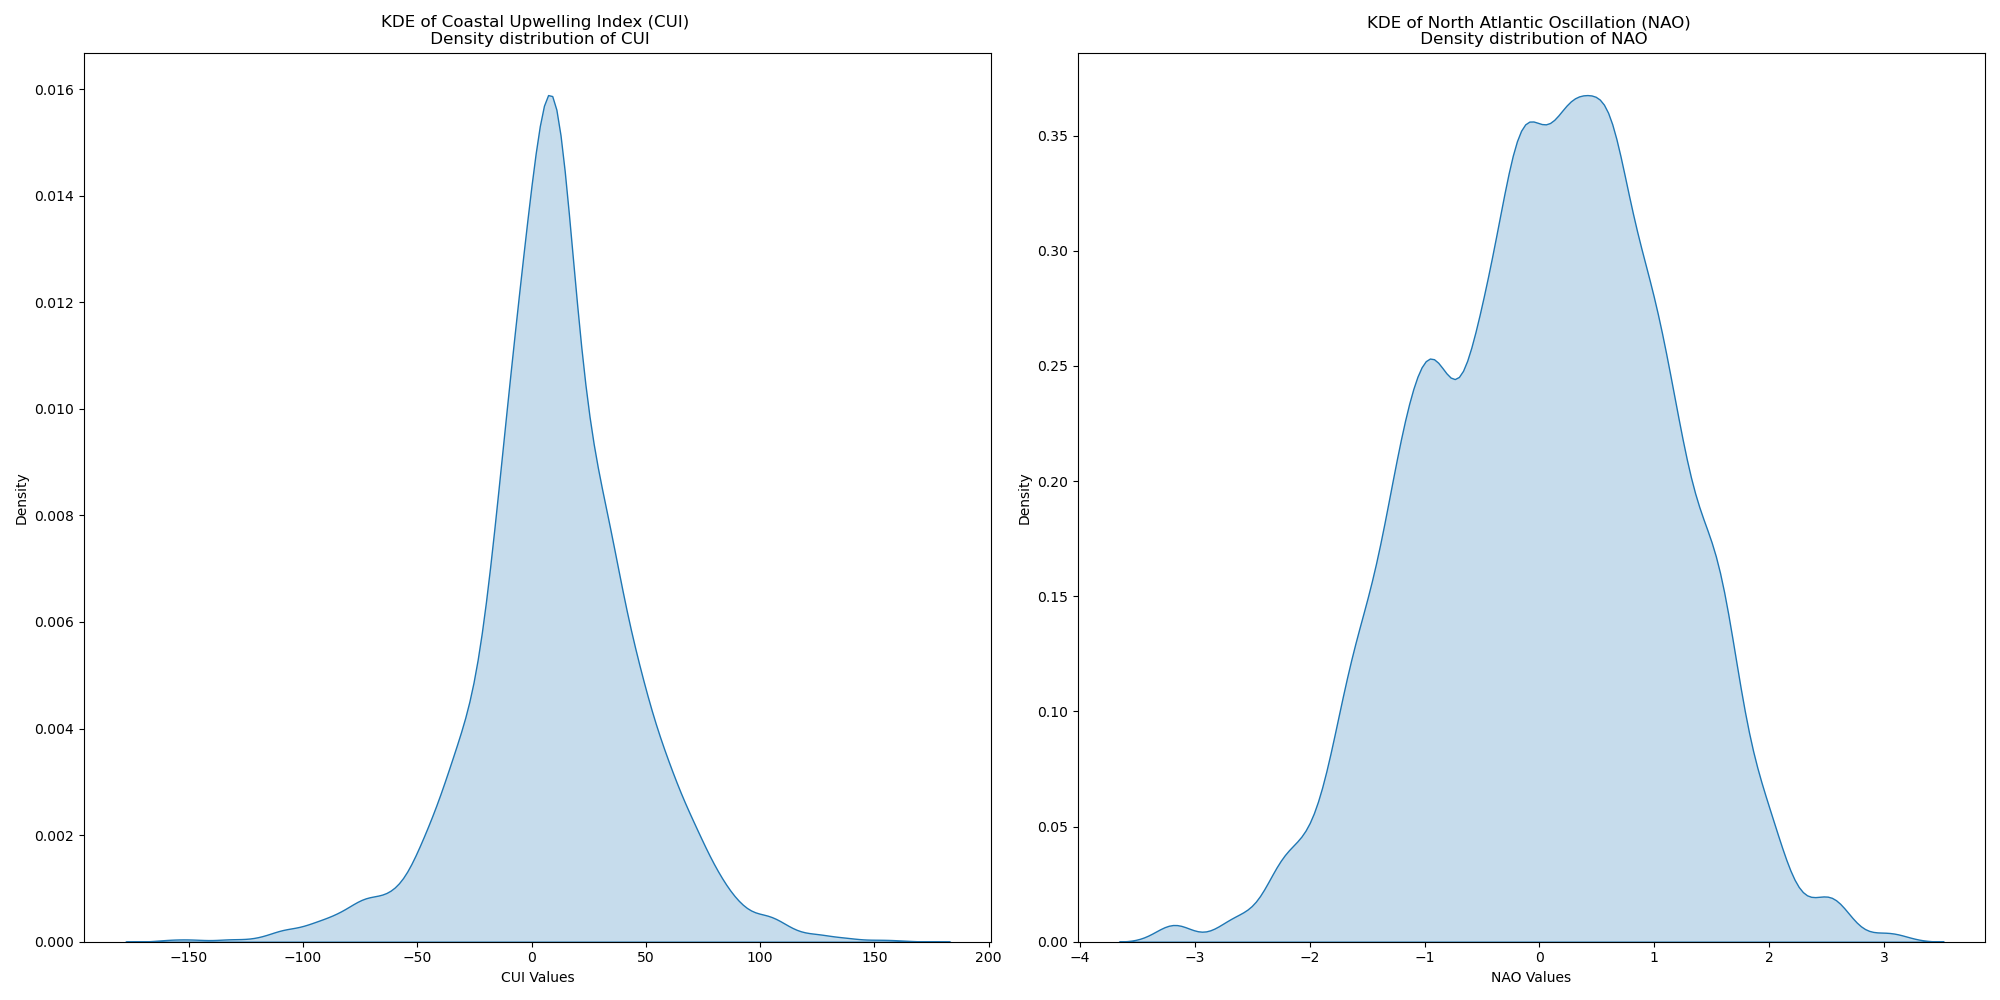
\includegraphics[scale=0.3]{kde_nao_cui.png}
\caption{distribution de probabilité pour NAO et CUI}
\end{figure}

"L'indice d'upwelling côtier (UI) et l'oscillation nord-atlantique (NAO) suivent tous deux une distribution normale avec des valeurs qui varient autour de 0, ce qui signifie que leurs valeurs sont symétriquement réparties autour d'une moyenne. Cela implique que les valeurs extrêmes (à la fois hautes et basses) sont moins fréquentes, et que la majorité des données se concentrent autour de cette moyenne."

\subsection{Analyse de la corrélation}
\begin{figure}[H]
\centering
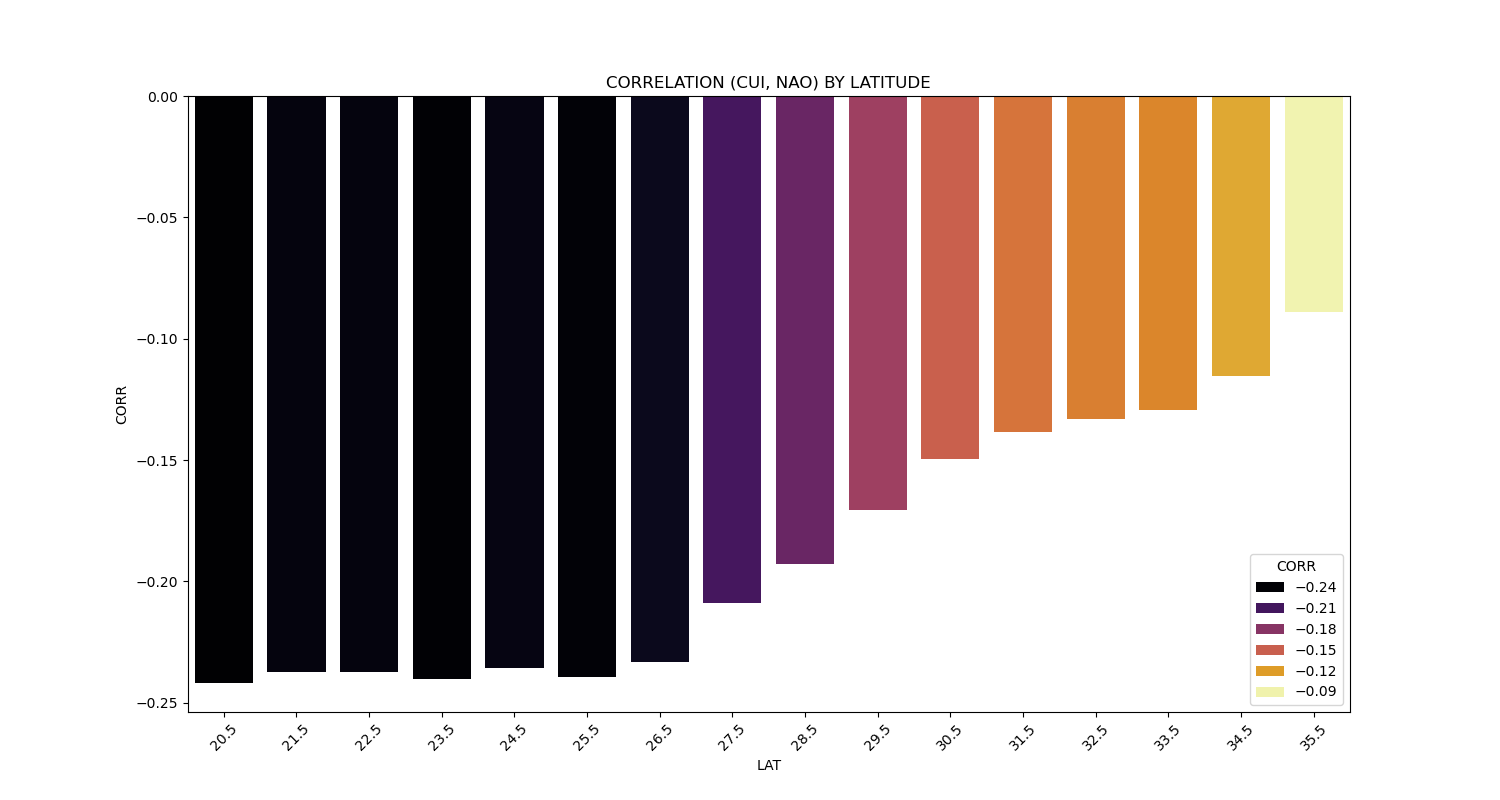
\includegraphics[scale=0.3]{corr.png}
\caption{Corrélation entre NAO et CUI par latitude}
\end{figure}

on remarque que la corrélation est généralement négative dans toutes les latitudes, toutefois, une remarque pertinente s'avère, c'est que la corrélation diminue  en module avec la latitude.

les basses latitudes (la zone sud du Maroc), connaissent une corrélation négative plus prononcée contrairement à la zone sud où la corrélation est presque nulle.

ces résultats confirme la réalité du Maroc avec une activité de pêcherie développée dans le sud motivée par les remontées des planctons causées par l'upwelling. 

\subsection{Analyse de l'Effet de NAO}

les résultats présents dans la figure ci-dessus confirme les résultats de la corrélation. Cette partie concerne l'analyse de l'Upwelling de façon séparée. en premier abord, analyser le CUI juste pour la phase positive de NAO, et en second abord, une analyse a concerné uniquement la phase négative de NAO.

\begin{figure}[H]
\centering
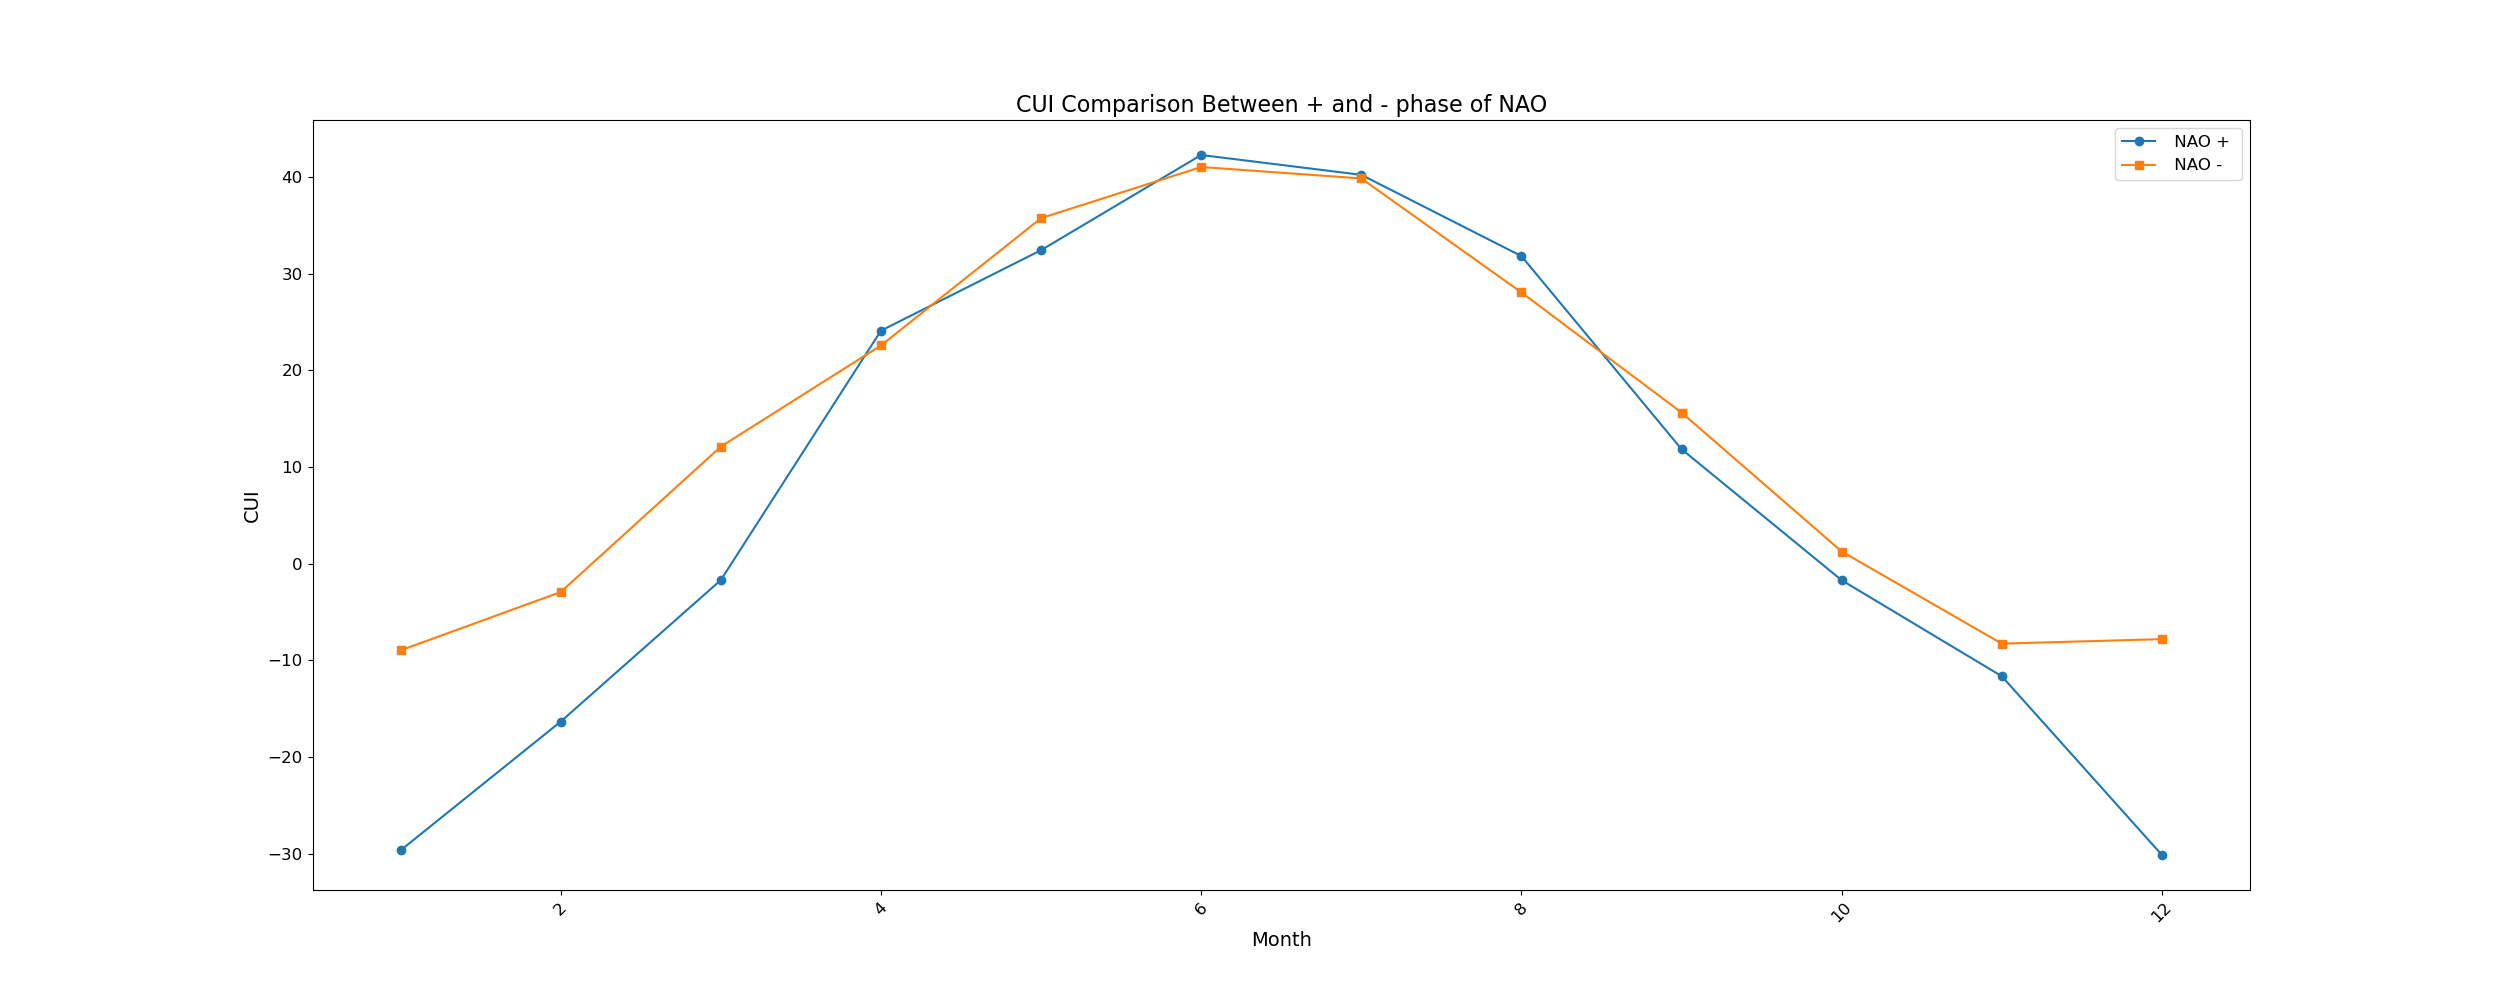
\includegraphics[scale=0.3]{CUI_NAO_PHASES.png}
\caption{Analyse de l'impact de la phase NAO sur le CUI.}
\end{figure}

le CUI au Maroc est caractérisé par une corrélation négative avec NAO, pour la phase positive de NAO on remarque que l'indice de l'upwelling côtier est inférieur au cas négatif de NAO. Ce résultat important exige une confirmation plus forte par une analyse de la climatologie du vent pour chaque phase de NAO.



\subsubsection{Phase Positive de NAO (NAO+)}


\begin{figure}[H]
\centering
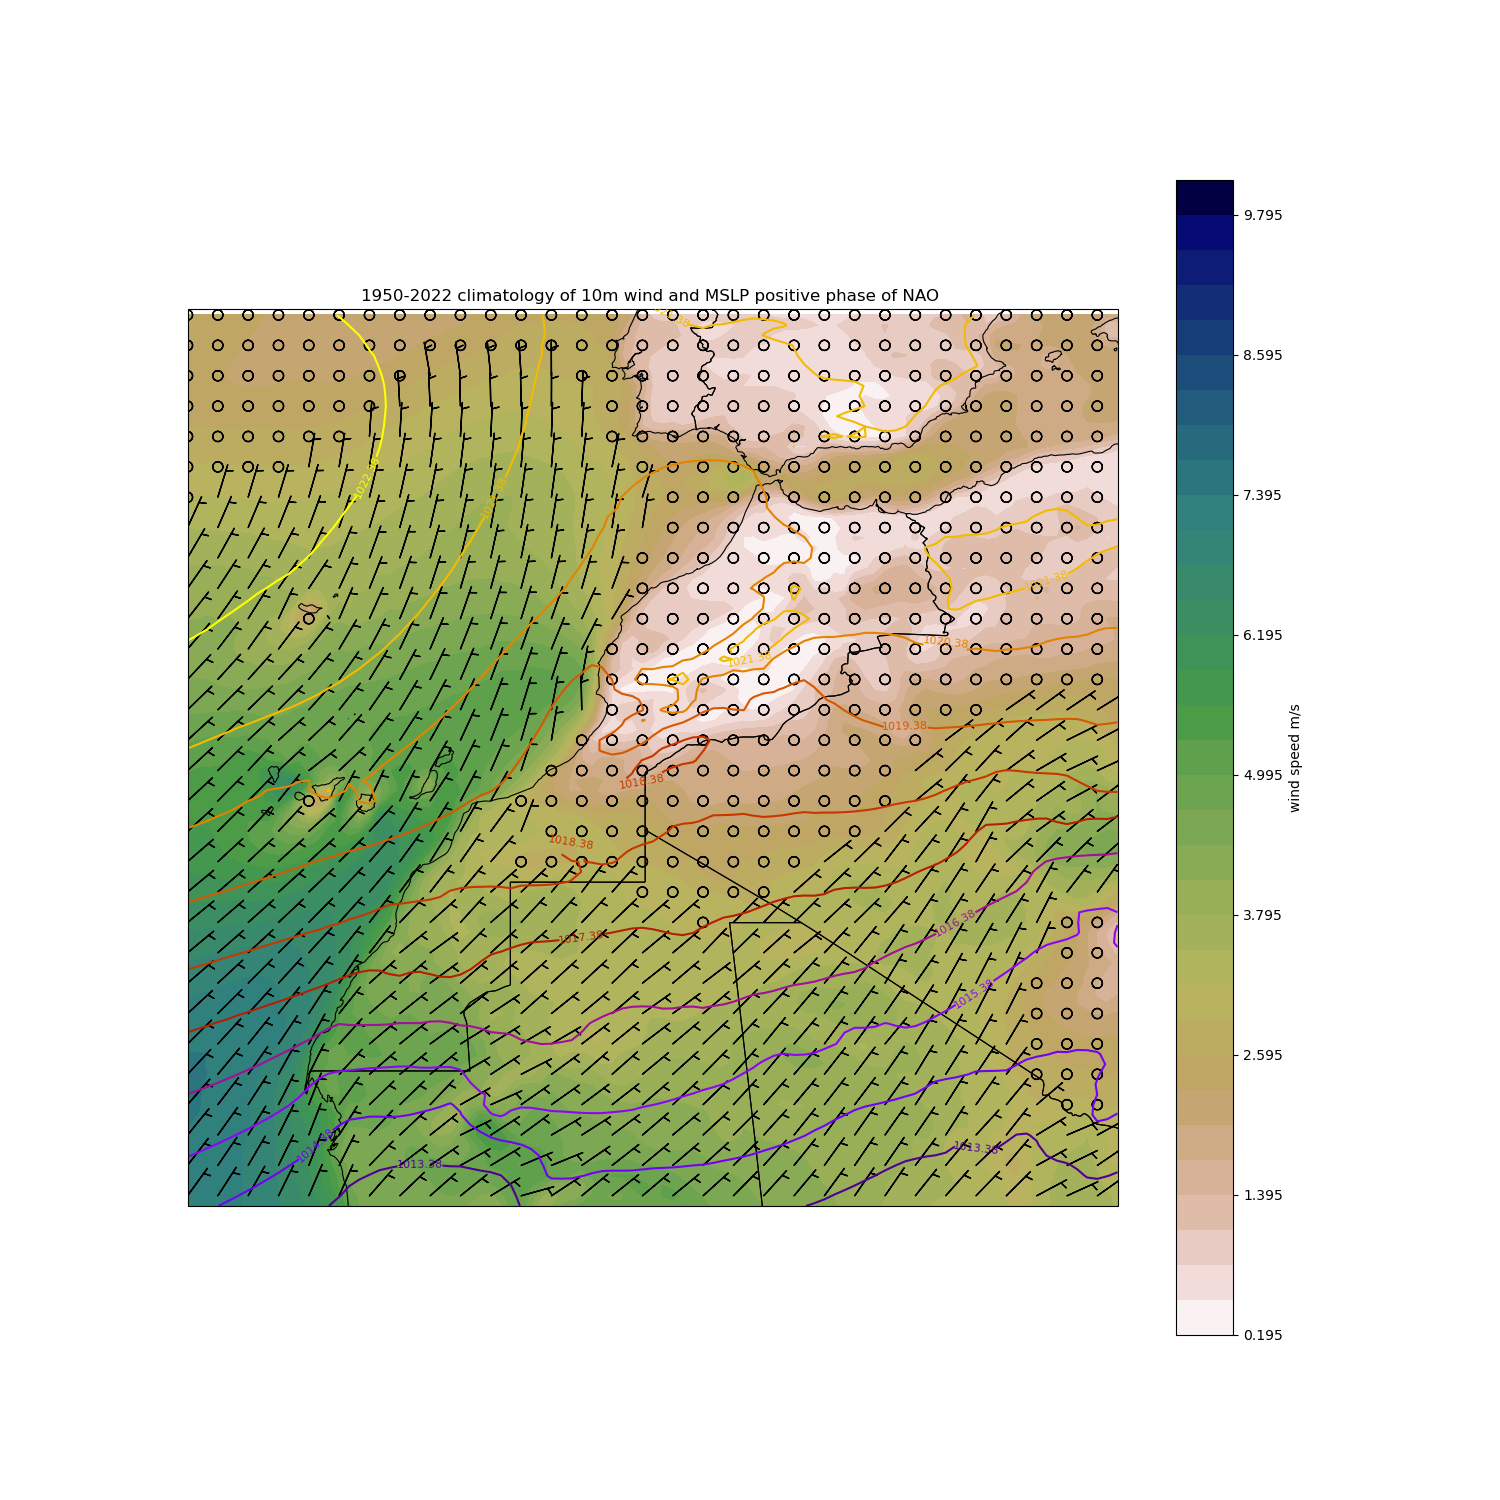
\includegraphics[scale=0.3]{POS_PHASE.png}
\caption{la climatologie du vent et de la pression pour la phase positive de NAO (1950-2022)}
\end{figure}


La phase positive de la NAO est associée à une intensité de vent relativement faible le long de la côte atlantique marocaine. Les caractéristiques principales observées dans cette phase sont :
\begin{itemize}
	\item \textbf {Direction du vent :} Les vents tendent à être moins bien alignés parallèlement à la côte, en particulier dans la zone sud. Cela peut réduire l’efficacité du mécanisme d’upwelling côtier (remontée d’eaux froides).
	\item \textbf{Intensité :} La vitesse moyenne du vent ne dépasse généralement pas 6 nœuds (environ 3 m/s). Cette faible intensité limite l’effet d’entraînement du vent sur les couches superficielles de l’océan, ce qui peut entraîner une diminution de l’upwelling, surtout dans les zones méridionales où ce phénomène est crucial pour les écosystèmes marins.
	\item \textbf{Implication sur le CUI :} Une phase NAO+ peut réduire la dynamique d’upwelling, impactant négativement la productivité marine et les activités de pêche dans la région.
\end{itemize}




\subsubsection{Phase Négative de NAO (NAO-)}


\begin{figure}[H]
\centering
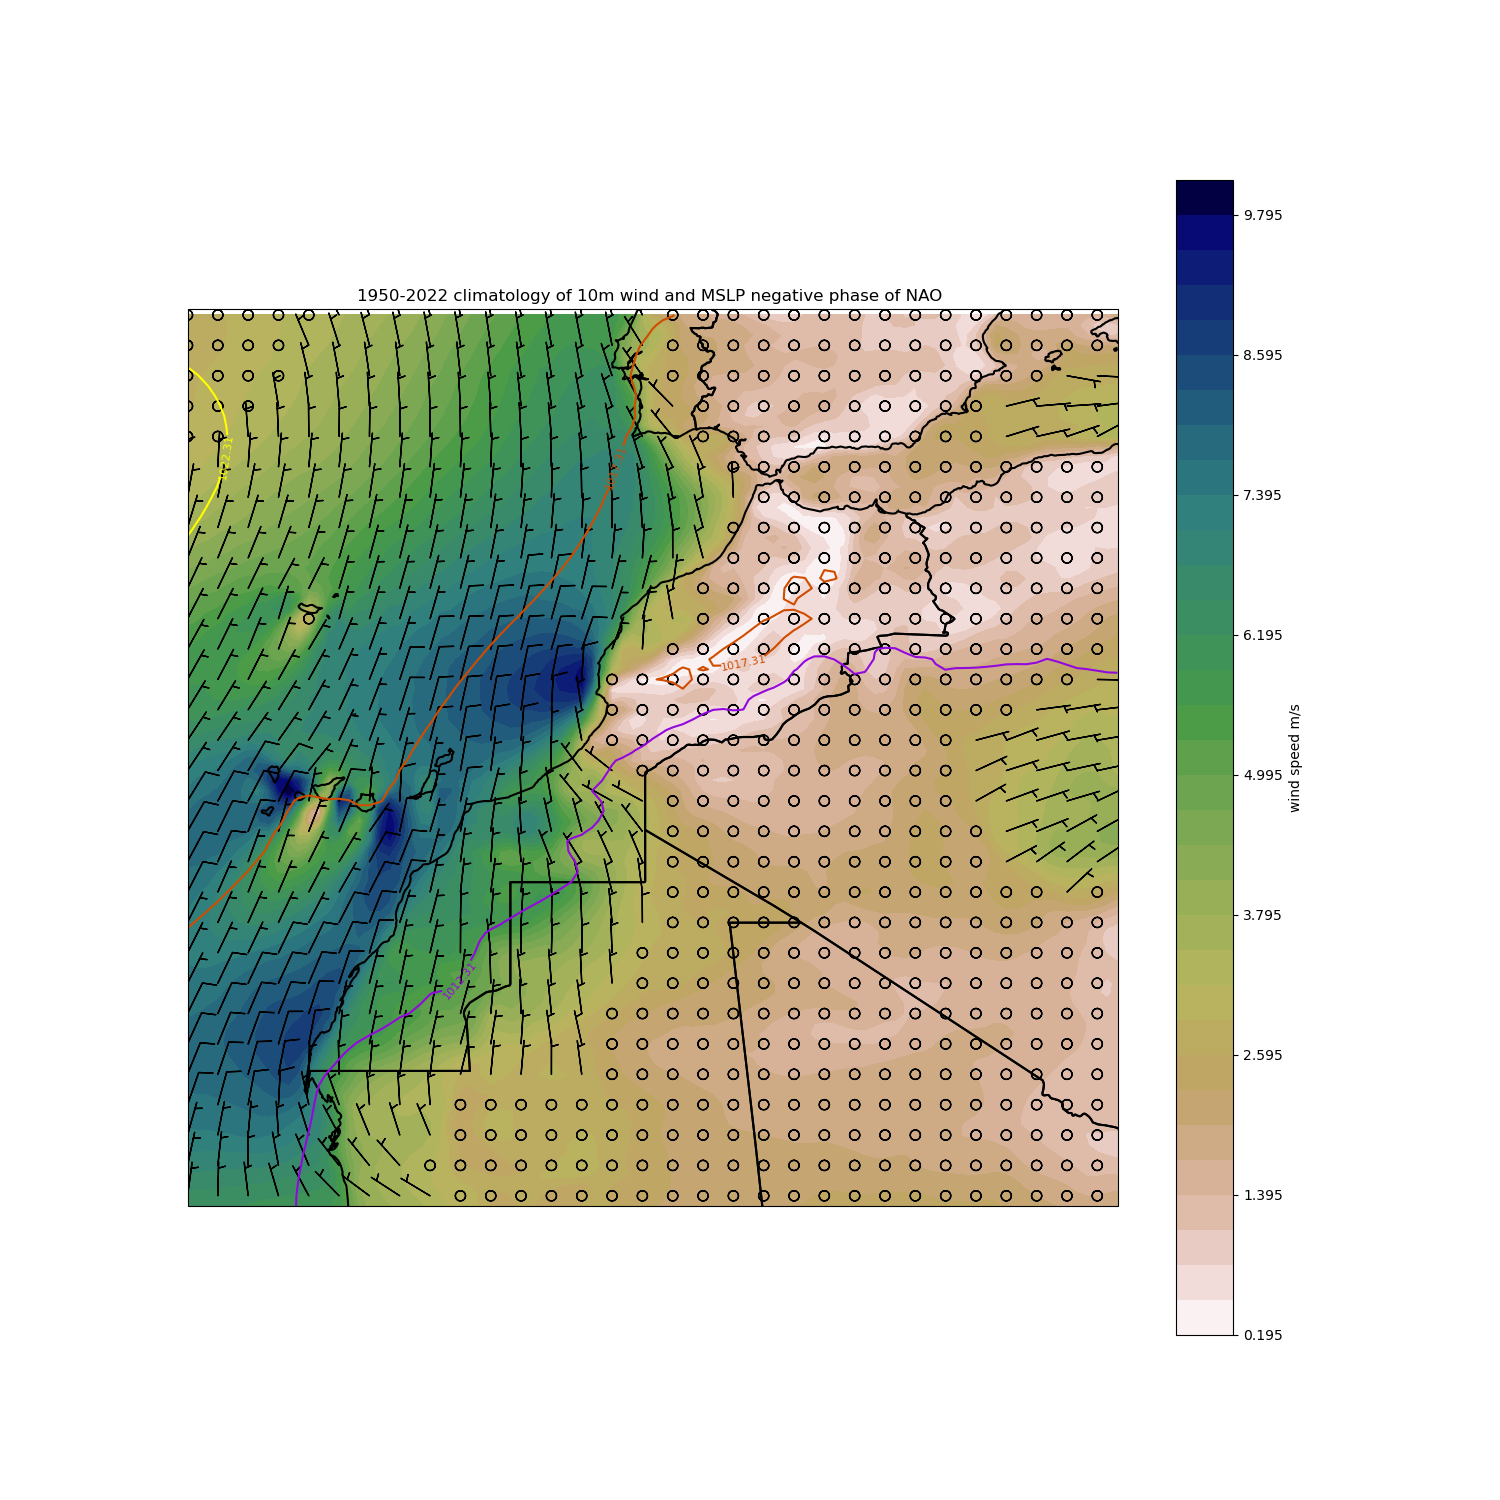
\includegraphics[scale=0.3]{NEG_PHASE.png}
\caption{la climatologie du vent et de la pression pour la phase négative de NAO (1950-2022)}
\end{figure}


La phase négative de la NAO se caractérise par des vents plus forts et mieux orientés le long de la côte atlantique, particulièrement dans les zones méridionales du Maroc. Les observations notables sont :
\begin{itemize}
	\item \textbf {Direction du vent :} Dans cette phase, les vents deviennent nettement parallèles à la côte, favorisant un upwelling côtier plus efficace. Cette configuration est particulièrement marquée dans les régions du sud, comme la zone située entre Agadir et Lagouira, où les vents suivent la ligne de côte de manière quasi parfaite.
	
	\item \textbf{Intensité :} La vitesse moyenne du vent atteint environ 10 m/s, soit bien supérieure à celle observée durant la phase positive. Cette intensité accrue renforce le transport d'Ekman, favorisant ainsi la remontée d’eaux froides riches en nutriments.
	
	\item \textbf{Implication sur le CUI :} Une phase $NAO - $ stimule fortement l’upwelling, augmentant la productivité biologique et soutenant les écosystèmes marins. Ces conditions peuvent être particulièrement bénéfiques pour les activités de pêche.
\end{itemize}


 
 